\section*{Ergebnisse}
\begin{itemize}
    \item Beschreiben und diskutieren Sie das Ergebnis Ihres Laborversuchs.
    \item Behauptungen, die aufgestellt werden müssen plausibel sein. Wenn sich bei der Messung etwas wesentlich schneller bewegt als in der Simulation ist die Begründung \glqq \textit{die Luftreibung wurde in der Simulation vernachlässigt}\grqq \ sehr selten korrekt.
    \item Stellen Sie Ihre Ergebnisse -- wenn sinnvoll -- grafisch dar. Ein Beispiel finden Sie in Abb.~\ref{fig:simulation_und_messung}. Ein Negativbeispiel, wie Bilder nicht ausschauen sollen finden Sie in Abb.~\ref{fig:negativbeispiel}. Achten Sie hier auch darauf die Zeitachse sinnvoll einzugrenzen und nur das zu Zeigen, was wirklich relevant ist.
    \item Die Diskussion der Ergebnisse soll den Versuch kritisch bearbeiten. Dazu ist eine Beschreibung und Berechnung der systematischen und statistischen Fehler notwendig.
\end{itemize}

%\begin{figure}[t]
%    \centering
%    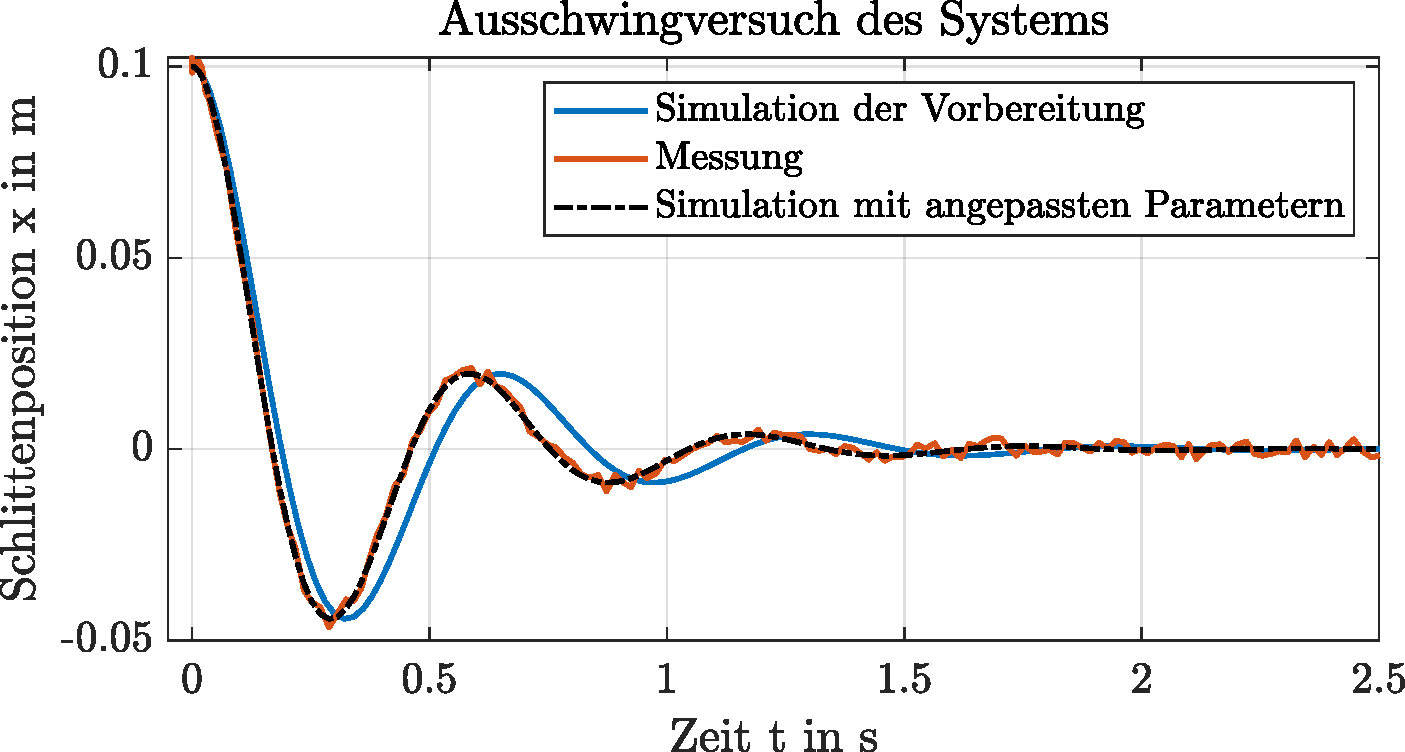
\includegraphics[width=0.95\linewidth]{images/Vergleich_Sim_und_Messung}
%	\caption{Beispielbild; Achten Sie \textbf{unbedingt} auf lesbare Achsenbeschriftungen und aussagekräftige Bildunterschriften. Referenzieren Sie auf Bilder im Text mit  Abb.~\ref{fig:simulation_und_messung}.}	   	
%	\label{fig:simulation_und_messung}
%\end{figure}

\begin{figure}[t]
	\centering
	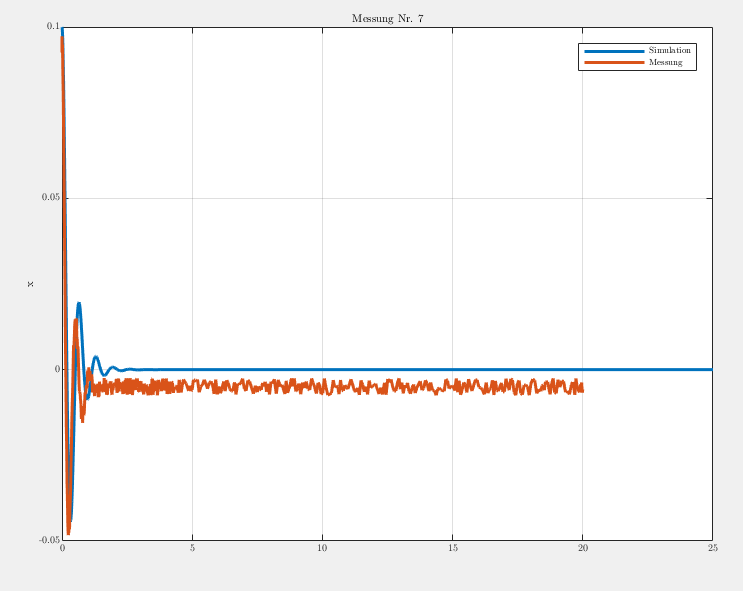
\includegraphics[width=0.95\linewidth]{images/Negativbeispiel}
	\caption{Für solche Bilder werden Negativpunkte vergeben.}	   	
	\label{fig:negativbeispiel}
\end{figure}